\documentclass[11pt]{report}
\usepackage[margin=1in, a4paper]{geometry}

\title{project2 frg report 2019}

\ifx\pdftexversion\undefined
\usepackage[dvips]{graphicx}
\else

\usepackage[pdftex]{graphicx}
\DeclareGraphicsRule{*}{mps}{*}{}
\fi
\graphicspath{ {./images/} }
\usepackage{url}
\usepackage{chapterbib}
\usepackage{hyperref}
\usepackage{lscape}
\usepackage{longtable}
\usepackage{float}
\usepackage{url}
\usepackage{multicol}
\usepackage{color}
\usepackage{fancyhdr}
\pagestyle{fancy}
\lhead{\leftmark}
\rhead{}
\lfoot{Micro-Cloud Setup Using OpenShift}
\rfoot{IIT Bombay}



\renewcommand{\bibname}{References}
\newcommand\tab[1][1cm]{\hspace*{#1}}

\setcounter{secnumdepth}{4}
\setcounter{tocdepth}{4}


\begin{document}
	
	\begin{titlepage}
		\begin{center}
			\Huge
			
			\textbf{Indian Institute of Technology
				Bombay} \\
			\ \\
			
			
			
\includegraphics[scale=1]{iitb}
			
			
			\textbf{Micro-Cloud Setup Using OpenShift}
			\ \\
			\ \\
			\Large
			Principal Investigator\\
			\textbf{Prof. S. Sudarshan }
			\ \\
			\ \\
			Project In-Charge\\
			\textbf{Mr. Nagesh Karmali}
			
			\ \\
			\ \\
			
			
			\Large
			\textbf{Project Team}
			\\
			\vspace{2cm}
			\textbf{Member1}
			\hspace{3cm}
			\textbf{Member2}
			\hspace{3cm}
			\textbf{Member3}
			\\
			Mr. Suraj Goel
			\hspace{1.2cm}
			Mr. Saurabh Vijay
			\hspace{1.cm}
			Ms. Anzum Bano\\
			\vfill
			
		\end{center}
	\end{titlepage}
	
	\pagebreak
	\begin{center}
		\Huge
		\ \\ \ \\ \ \\
		\textbf{Summer Internship 2019} \\
		\ \\
		\textbf{Project Approval Certificate}    
		\ \\
		\Large
		\textbf{Department of Computer Science and Engineering} \\
		\textbf{Indian Institute of Technology, Bombay} \\
		\ \\ \ \\
		
		The project entitled submitted by Mr. Suraj Goel, Mr. Saurabh Vijay, Ms.
		Anzum Bano is approved for Summer Internship 2019 programme from 20th
		May 2019 to 9th July 2019, at Department of Computer Science and Engineering, IIT
		Bombay.
		\ \\
		\ \\
		\  \\
		\ \\
		\ \\
		\ \\ 
		\ \\
	
		
		
	\end{center}
				\rule{180pt}{1pt}
			\hspace{1.5cm}
			\rule{180pt}{1pt} 
			\\
			\Large
			\textbf{Prof. S. Sudarshan}
			\hspace{3.0cm}
			\Large
		    \textbf{Mr. Nagesh Karmali}
			\\
			Dept. of CSE, IIT Bombay
			\hspace{2.0cm}
			Sr. Project Manager (Research)
			\\
			Principle Investigator
			\hspace{3.2cm}
			Dept. of CSE, IIT Bombay
		
			
			
			
	
	\pagebreak
	
	
	\begin{center}
		\Huge
		\textbf{Declaration} \\
		\ \\
		\Large
		I declare that this written submission represents my ideas in my own words and where
		others’ ideas or words have been included, I have adequately cited and referenced the
		original sources. I also declare that I have adhered to all principles of academic
		honesty and integrity and have not misrepresented or fabricated or falsified any
		idea/data/fact/source in my submission. I understand that any violation of the above
		will be cause for disciplinary action by the Institute and can also evoke penal action
		from the sources which have thus not been properly cited or from whom proper
		permission has not been taken when needed.\\
		\ \\
		\ \\
		\ \\
		\ \\
		\ \\
		\ \\
		\ \\ 
		\ \\
		\ \\
		\ \\
		\textbf{Suraj Goel}
		\hfill
		\textbf{ Saurabh Vijay} 
		\hfill
		\textbf{Anzum Bano}\\
		MNNIT Allahabad
		\hfill
		MNNIT Allahabad
		\hfill
		MNNIT Allahabad
		
		\begin{flushleft}
			\vspace{2.5cm}
			\textbf{Date}\\
		\end{flushleft}
	\end{center}
	
	
	
	\pagebreak
	
	\begin{center}
		\huge
		
		\textbf{ACKNOWLEDGEMENT}
	\end{center}
	\vspace{3cm}
	
	\large
	We, the summer interns of this group, are overwhelmed in all humbleness and
	gratefulness to acknowledge our deep gratitude to all those who have helped us put
	our ideas to perfection and have assigned tasks well above the level of simplicity and
	into something concrete and unique.
	We,  wholeheartedly thank ​ Mr. Nagesh Karmali ​ for providing us the opportunity to work on this
	project.He was and is always there to show us the right track when needed help.
	With help of his brilliant guidance and encouragement, we all were able to complete
	our tasks properly and were up to the mark in all the tasks assigned.Our sincere thanks to
	Mrs. Anjali , Mr. Gaurav Patil and Mr. Gaurav Ojha without whom the project would not have been
	successful .
	 During the
	process, we got a chance to see the stronger side of our technical and nontechnical
	aspects and also strengthen our concepts.
	Last but not the least, we wholeheartedly thank all our other colleagues working in
	different projects under ​ Prof. S.Sudarshan for helping us evolve better with their
	critical advice.
	
	\pagebreak
	
	\begin{center}
		\huge
		
		\textbf{ABSTRACT}
	\end{center}
	\vspace{3cm}
	Micro-cloud Setup using openshift is aimed to provide an open source cloud-based user-friendly platform, which can be used to create, test, and run applications, and                    
	finally deploy them on cloud.
	Moreover, this project is capable of managing applications smoothly, written in various languages, such as Node.js, Ruby, Python, Perl, and Java. 
	\ \\
	One of the key features of this project, being focussed on OpenShift is, it is extensible, which helps the users support the application written in other languages.
	additionally, this project provides a common platform for enterprise units to host their applications on cloud without worrying about the underlying operating system. This makes it very easy to use, develop, and deploy applications on cloud. One of the key features is, it provides managed hardware and network resources for all kinds of development and testing. With OpenShift,this project gives PaaS developer the complete freedom to design their required environment with specification.
	\listoffigures
	\tableofcontents
	
	\pagebreak
	
	\chapter{INTRODUCTION}
	\large
	Micro-cloud setup using Openshift technology is the project undertaken by Eklavya summer internship program at IIT Bombay, which focuses on OpenShift Container Platform a microservices-based architecture of smaller, decoupled units that work together.
	\
	
	\
	It runs on top of a Kubernetes cluster, with data about the objects stored in etcd, a reliable clustered key-value store.
	\
	
	\
	The Docker service provides the abstraction for packaging and creating Linux-based, lightweight container images and the Kubernetes provides the cluster management and orchestrates containers on multiple hosts.
	
	\textbf { OpenShift Container Platform adds:}
	\begin{itemize}
		\large
		\item Source code management, builds, and deployments for developers.
		\item Autoscaling and Automatic load balancing in an application.
		\item Managing and promoting images at scale as they flow through your system.
		\item Team and user tracking for organizing a large developer organization.
		\begin{figure}[h!]
    	\begin{center}
    		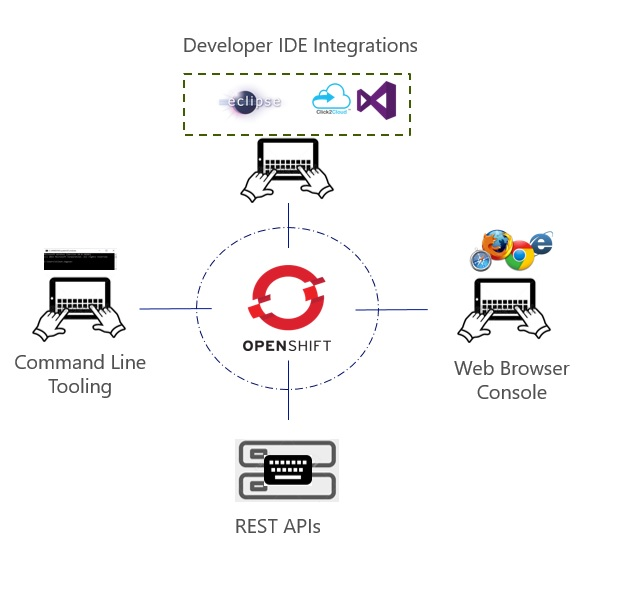
\includegraphics[width=0.80\textwidth, totalheight=0.30\textheight]{intro.png}
    		\caption{OpenShift Layout \cite{intro}}
    	  \end{center}
	  
		\end{figure}
		
		
	\end{itemize}
	\large
	\pagebreak
	\section{Purpose}
	\
	\
	\begin{itemize}
		\large
		\item To provide a platform so that both Developers and Operators can work together without having to sacrifice their individual concerns.
		\vspace{0.3cm}
		\item Since deploying and managing containers at scale is a complicated process, OpenShift enables efficient container orchestration, allowing quicker container provisioning, deploying, scaling, and management.
		\vspace{0.3cm}
		\item To allow applications to migrate their container processes to the new operating system quickly, while avoiding the extensive costs often involved in migrating.
		\vspace{0.3cm}
		\item To automate the process of building new container images for all of your users. So that standard Docker builds based on the Dockerfiles manually provided can be run, and also provide a “Source-to-Image” feature which allows to specify the source from which image is to be generated.
		\large
	\end{itemize}
	\large
	\section{Scope}
	\large
	The target audience of our project is not limited to any particular group or system rather the
	module(project) is compatible with every web application. This
	module can be used in context with any web application for creating, deleting ,managing, deploying etc.
	\pagebreak
	\LARGE
	
	\chapter{Motivation}
	\vspace{1cm}
	\large
	\begin{itemize}
		\item
		With OpenShift, developers have access to a self-service platform that allows them to create, modify, and deploy applications on demand with the click of a button .
		\vspace{0.3cm}
		\item 
		applications should be incredibly portable and hyper scalable.OpenShift's orchestration layer, Google’s Kubernetes, automates the scheduling and replication of these containers meaning that they're highly available and able to accommodate whatever your users can throw at it.
		\vspace{0.3cm}
		\item
		Data should be protected from any type of harm.OpenShift is built on those same principles and applications running on OpenShift have their own "container"allowing for the code and data to separated from each other by default.
		\vspace{0.3cm}
		\item
		IT organizations need a vendor that can enable them through the entire stack, not just one aspect of it. Having a PaaS environment that’s coupled together with supported IaaS services and middleware services, means better agility and interoperability.
		\vspace{0.3cm}
		\item
		Operations needs to be able to maintain those applications easily and have them run at the appropriate scale. OpenShift enables them to do that with little to no manual intervention
	\end{itemize}
	\section{Objective}
	Setting up Micro-cloud architecture with commodity storage and server nodes using OpenShift(PaaS). OpenShift will provide infrastructure for orchestration of dockerized images of applications like Open edX/ IITBombayX/Moodle/Drupal.
	
	\begin{itemize}
		\item Giving access to developer to create , modify and deploy applications on demand with the click of a button .
		\item To increase portability of applications by containerizing phenomena . 
		\item To Make applications more scalable so that they can be scaled according to the traffic of users
		\item To make applications more reliable and secure by containerize code and data separately .
		\item Single click installation of applications despite of any kind of OS .
	\end{itemize}
	\vspace{0.8cm}
	\section{Technologies Used}
	\vspace{0.8cm}
	\begin{itemize}
		\item 
		\textbf{Openshift} : OpenShift is an open source hybrid cloud application Platform as a Service (PaaS) .
		\item
		\textbf{Docker} : Docker is an open source software platform to create, deploy and manage virtualized application containers on a common operating system (OS), with an ecosystem of allied tools.
		\item
		\textbf{Kubernetes} : Kubernetes (K8s) is an open-source system for automating deployment, scaling, and management of containerized applications .
		\item
		\textbf{Shell Scripting} : 
		A shell script is a text file that contains a sequence of commands for a UNIX-based operating system.
		\item
		\textbf{MySql} : It is used for provisioning different services and to provide database for different services .
		\item
		\textbf{Git} : Git is a free and open source distributed version control system designed to handle everything from small to very large projects with speed and efficiency. Git repositories contain
		source code for different application and services .
	\end{itemize}
	
	
	\pagebreak
	
	
	\chapter{Open edX Platform}
	\section{Introduction}
	openedX is an open source online MOOC platform to create and deliver online courses.\ \\
	This chapter deals with the various aspects of openedX such as the key components,Versions of openedX available and Steps of Installation.
	\section{Open edX Versions}
	\begin{itemize}
		\large
		\item  \textbf{Ginko}
		\item  \textbf{Hawthorn}
		\item  \textbf{Ironwood}
	\end{itemize}
	\section{Types Of Installations}
	\begin{itemize}
		\large
		\item \textbf{Native Installation} \ \\
		The Native installation installs the Open edX software on your own Linux machine in a production-like configuration. Details are at the Open edX Native Installation page on the edX wiki. \ \\
		\underline{\href{https://openedx.atlassian.net/wiki/spaces/OpenOPS/pages/146440579/Native+Open+edX+Ubuntu+16.04+64+bit+Installation}{Installation Wiki}}
		
		\item \textbf{Docker Based Installation} \ \\
		The Docker Based Installation is done using Open edX Devstack.
		Devstack is a deployment of the Open edX platform within a set of Docker containers designed for local development. Running the Open edX platform locally allows you to discover and fix system configuration issues early in development.
	\end{itemize}
	\pagebreak
	\section{openedX Components}
	\large
	Few key Components of openedX:
	\begin{itemize}
		\item \textbf{Learning Management System (LMS)} \ \\
		The LMS is the most visible part of the Open edX project. Learners take courses using the LMS. The LMS also provides an instructor dashboard that users who have the Admin or Staff role can access by selecting Instructor. \ \\
		The LMS uses a number of data stores. Courses are stored in MongoDB, with videos served from YouTube or Amazon S3. Per-learner data is stored in MySQL.
		\item \textbf{Studio} \ \\
		Studio is the course authoring environment. Course teams use it to create and update courses. Studio writes its courses to the same Mongo database that the LMS uses.
		\item \textbf{Forum} \ \\
		The LMS uses an API provided by the comments service to integrate discussions into the learners’ course experience.
		\item \textbf{Elastic Search} \ \\
		The Open edX project uses Elasticsearch for searching in multiple contexts, including course search and the comments service.
		
	\end{itemize}
	\section{Steps Of Installation}
	\large
	The following steps installs the ironwood-release of devstack 
	\begin{itemize}
		\item git clone https://github.com/edx/devstack
		\item cd devstack
		\item git checkout open-release/ironwood.master
		\item export OPENEDX RELEASE=ironwood.master
		\item make dev.checkout
		\item make dev.clone
		\item make dev.provision
	\end{itemize}
	
	\section{Errors Faced In Installation}
	\begin{itemize}
		\item \textbf{./provision.sh: line 21: /usr/local/bin/docker-compose: Permission denied} \ \\
		Makefile:59: recipe for target 'dev.provision.run' failed \ \\
		make: *** [dev.provision.run] Error 126 \ \\
		Solution : \ \\
		$ sudo -i  \ \\
		$ curl -L \ \\ https://github.com/docker/compose/releases/download/1.18.0/docker-compose-`uname -s`-`uname -m` -o /usr/local/bin/docker-compose \ \\
		$ chmod 755 /usr/local/bin/docker-compose \ \\
		$ exit \ \\
		
		\item \textbf{TASK [common : Update expired apt keys] **************} \ \\
		This error occurs due to the fetching to apt-keys from an expired link. \ \\
		Solution : \ \\
		1.sudo exec -it edx.devstack.lms bash \ \\
		2.cd app/edx\_ansible/edx\_ansible/playbooks/roles/common\_vars/defaults/ 
		3.vi main.yml \ \\
		4.On entering the main.yml file in vim editor change the link for the keyword
		COMMON\_EDX\_PPA\_KEY from keyserver.ubuntu.com to  hkp://keyserver.ubuntu.com:80 \ \\
	\end{itemize}
	
	\section{Docker Containers after Installation}
	\begin{table}[H]
		\begin{center}
			\begin{tabular}{|c|c|p{7cm}|}
				\hline
				\textbf{No.} & \textbf{Container Name} & \textbf{Docker Image} \\
				\hline
				1 & edx.devstack.chrome & edxops/chrome:ironwood.master  \\
				\hline
				2 & edx.devstack.elasticsearch & edxops/elasticsearch:devstack \\
				\hline
				3 & edx.devstack.firefox & edxops/firefox:ironwood.master \\
				\hline
				4 & edx.devstack.memcached & memcached.devstack.edx \\
				\hline
				5 & edx.devstack.mongo & mongo:3.2.16 \\
				\hline
				6 & edx.devstack.mysql & mysql:5.6 \\
				\hline
				7 & edx.devstack.credentials & edxops/credentials:ironwood.master \\
				\hline
				8 & edx.devstack.discovery & edxops/discovery:ironwood.master \\
				\hline
				9 & edx.devstack.ecommerce & edxops/ecommerce:ironwood.master \\
				\hline
				10 & edx.devstack.lms & edxops/edxapp:ironwood.master \\
				\hline
				11 & edx.devstack.edx\_notes\_api & edxops/notes:ironwood.master \\
				\hline
				12 & edx.devstack.studio & edxops/edxapp:ironwood.master \\
				\hline
				13 & edx.devstack.forum & edxops/forum:ironwood.master \\
				\hline
				14 & edx.devstack.devpi & edxops/devpi:ironwood.master \\
				\hline
				15 & edx.devstack.gradebook & node:10 \\
				\hline
				
			\end{tabular}
			\caption{Containers}
		\end{center}
	\end{table}
	
	
	\large
	Follow below links for more information: \ \\
	\href{https://github.com/fresearchgroup/Micro-Cloud-setup-using-Openshift-on-commodity-servers/blob/master/openedX\_Devstack\_Installation/Installation\%20steps\%20and\%20Errors.docx}{Installation Steps}
	\ \\
	\href{https://github.com/fresearchgroup/Micro-Cloud-setup-using-Openshift-on-commodity-servers/blob/master/openedX\_Devstack\_Installation/Explanation\%20Ironwood\_Docker\%20Installation.docx}{Installation Explanation}
	
	\pagebreak
	\chapter{Setting Up Openshift on Commodity Servers}
	\section{OpenShift-Fundamentals}
	OpenShift is an open source hybrid cloud application Platform as a Service (PaaS). Community version of openshift is OKD. Major Components of Openshift are :- 
	\\
	\\
	\begin{enumerate}
		
		\item 
		\textbf{Docker} : Docker is an open-source software tool designed to automate and ease the process of creating, packaging, and deploying applications using an environment called a container.
		\\
	\begin{figure}[h!]
    	\begin{center}
    		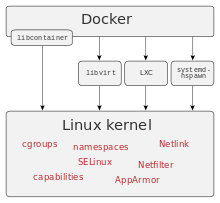
\includegraphics[scale=0.7]{docker.png}
    		\caption{Docker \cite{Docker}}
    	  \end{center}
	  
		\end{figure}
		\ \\
		\ \\
		\large
		\textbf{Docker Terminology}:
		\begin{itemize}
			\item
			\textbf{Docker Container}: A Docker Container encapsulates a Docker image and when live and running, is considered a container. Each container runs isolated in the host machine.
			\begin{figure}[h!]
    	\begin{center}
    		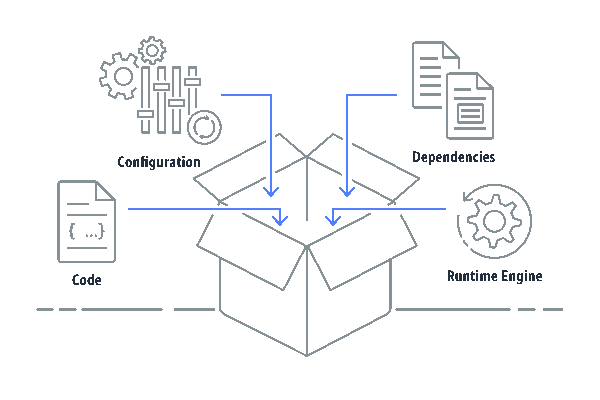
\includegraphics[scale=0.3]{containerization.png}
    		\caption{Container \cite{container}}
    	  \end{center}
	  
		\end{figure}
			\item
			\textbf{Docker Image}: A Docker Image is the basic unit for deploying a Docker container. A Docker image is essentially a static snapshot of a container, incorporating all of the objects needed to run a container.
			
			\item \textbf{Containerization} : Containerization is a lightweight alternative to full machine virtualization (like VMWare) that involves encapsulating an application within a container with its own operating environment.
			\ \\
			\ \\
			
			\item
			\textbf{Docker Registry}:The Docker Registry is a stateless, highly scalable server-side application that stores and distributes Docker images. 
			\ \\
			\ \\
			\item
			\textbf{Docker Engine}: The Docker Engine is a layer which exists between containers and the Linux kernel and runs the containers.
			\\
			\begin{figure}[h!]
    	\begin{center}
    		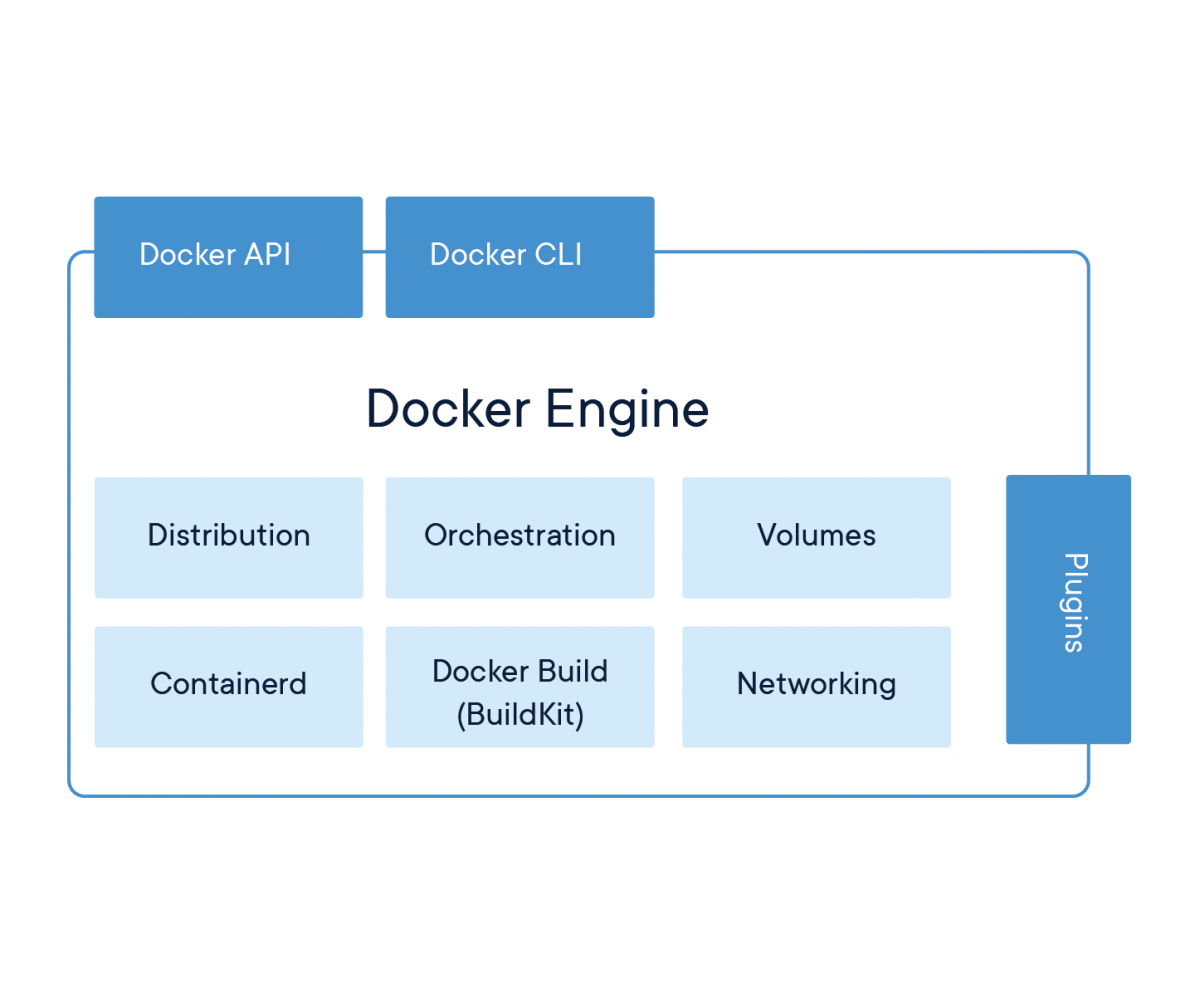
\includegraphics[scale=0.4]{docker-engine.png}
    		\caption{Docker Engine \cite{DockerEngine}}
    	  \end{center}
	   \end{figure}
			
			
			\ \\
			\item
			\textbf{Dockerfiles}: Dockerfiles are merely text documents (.yaml files) that contains all of the configuration information and commands needed to assemble a container image.
			\item
			\textbf{Docker Compose}: Docker Compose is a tool that defines, manages and controls multi-container Docker applications. With Compose, a single configuration file is used to set up all of your application’s services .
			
			
		\end{itemize}
		\item
		\textbf{Kubernetes}:Kubernetes is a container-orchestration tool which provides a smart way for orchestration in setting a multi-node cluster.Kubernetes comes with a lot of functionalities such as load balancing, pod scaling, process scheduling and process management.
		\\
		\\
		\\
		\begin{figure}[h!]
    	\begin{center}
    		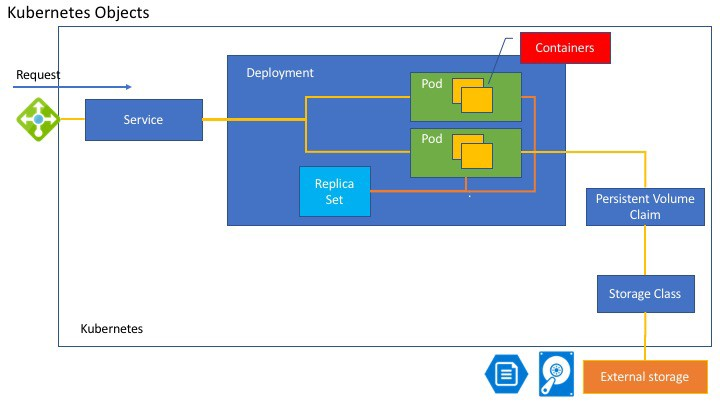
\includegraphics[scale=0.5]{kubernetes.jpeg}
    		\caption{Kubernetes Architecture \cite{kubearch}}
    	  \end{center}
	  
		\end{figure}
		\\
		\\
		\\
		\textbf{Kubernetes Terminology}:
		\begin{itemize}
			\item
			\textbf{Pods} : The most fundamental unit in a kubernetes cluster is a pod. A pod is a collection of container and volumes. Each pod has an IP address. 
			\\
			\\
			\item
			\textbf{Deployment} : A deployment can be seen as a stateless state of the pod. A deployment is used to provide pod definition and rolling updates to the pod. A deployment contains information such as number of replicas, image, volume .
			\\
			\\
			\\
			\\
		\begin{figure}[h!]
    	\begin{center}
    		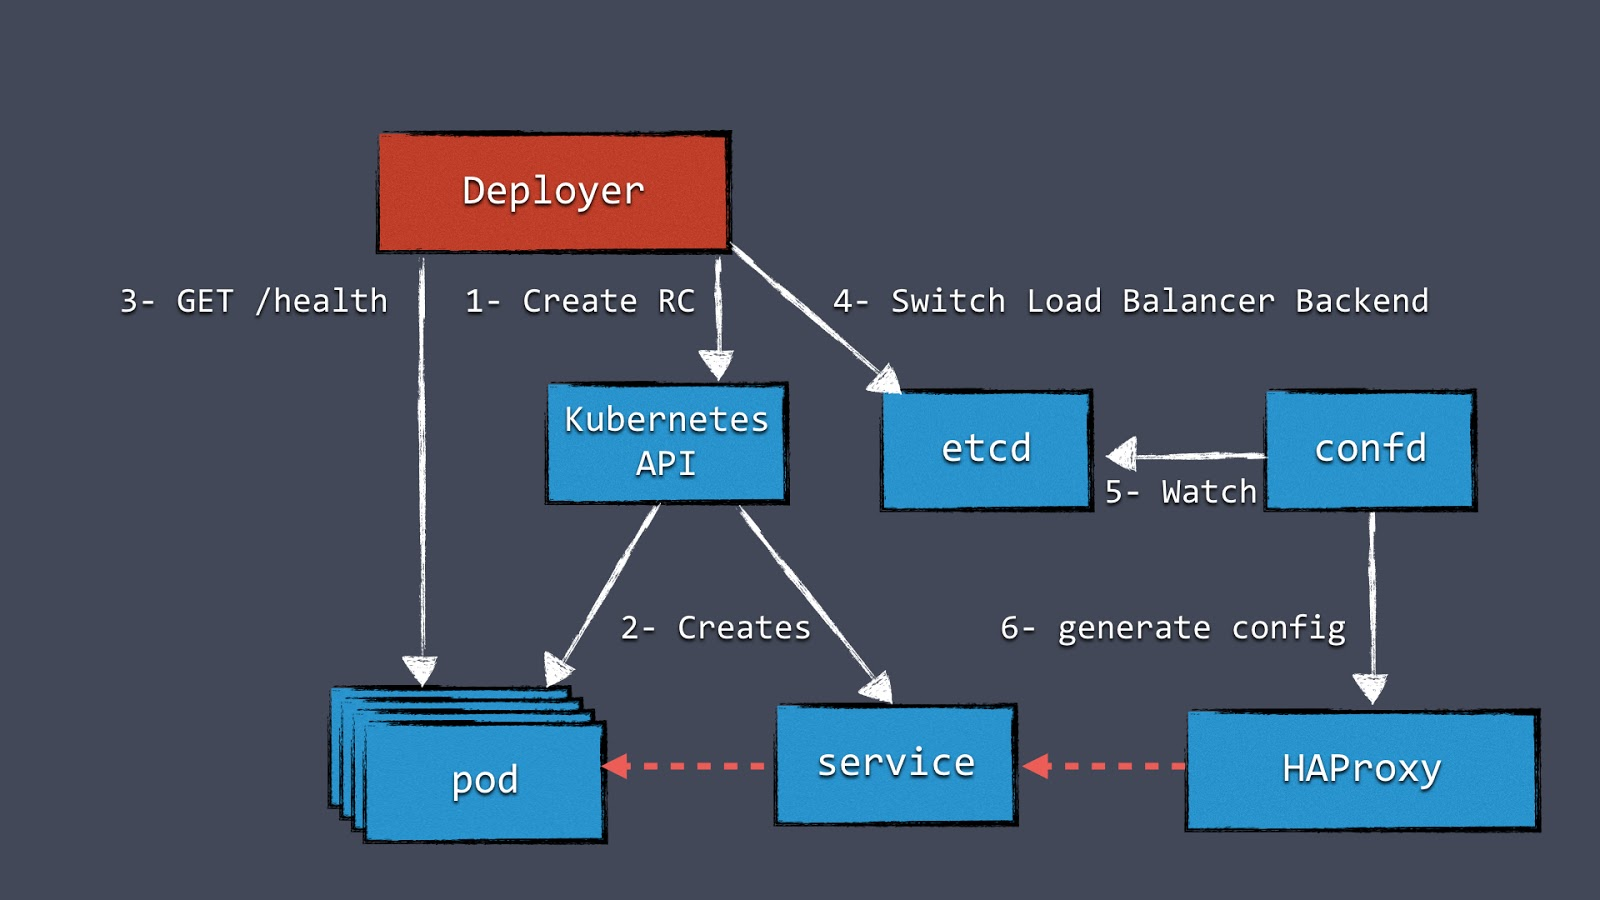
\includegraphics[scale=0.25]{deployment.jpeg}
    		\caption{Kubernetes Deployment \cite{kubedep}}
    	  \end{center}
	  
		\end{figure}
			\\
			\\
			\\
			\item
			\textbf{Service} : A service exposes a deployment as a network service. A deployment is stateless whereas a service can be considered as a stateful definition. The three types of services in kubernetes are : ClusterIP, NodePort and LoadBalancer. 
			\\
			\\
			\item
			\textbf{Ingress Network}: An ingress network exposes the services in the cluster to the outside network i.e. the clients.
			\\
			\begin{figure}[h!]
    	\begin{center}
    	    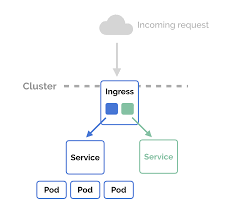
\includegraphics[scale=0.6]{ingress.png}
    		\caption{Ingress Network \cite{Ingress}}
    	  \end{center}
	  
		\end{figure}
			
		\end{itemize}
	\end{enumerate}
	\pagebreak
	\section{Openshift Architecture}
	OpenShift uses the kubernetes master/node architecture as a starting point .\ \\
	\ \\
	\ \\
	Apart from k8s architecture, OpenShift has the following parts:
	\ \\
	\begin{itemize}
		\item\textbf{ Routing layer}:
		The routing layer is a software load balancer.When an application is deployed, a DNS entry is created for it automatically.
		\vspace{1cm}
		
		\item\textbf{Integrated container registry}:An image registry is a central location that can serve container images to multiple locations.In addition to providing tightly integrated image access,Openshift works to provide more efficiency.
		\ \\
		\ \\
		\ \\
		\begin{figure}[h!]
    	\begin{center}
    	    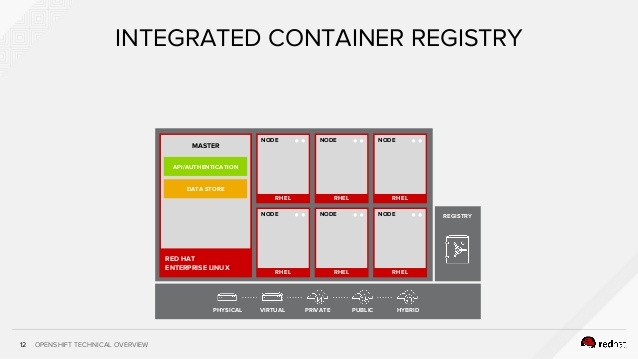
\includegraphics[scale=0.75]{openshiftimageregistry.jpg} 
    		\caption{Integrated Container Registry\cite{Intreg}}
    	  \end{center}
	  
		\end{figure}
		
		\ \\
		\ \\
	\end{itemize}
	\pagebreak
	\textbf{Openshift Cluster OverView}
	\vspace{2cm}
	\begin{figure}[h!]
    	\begin{center}
    	   		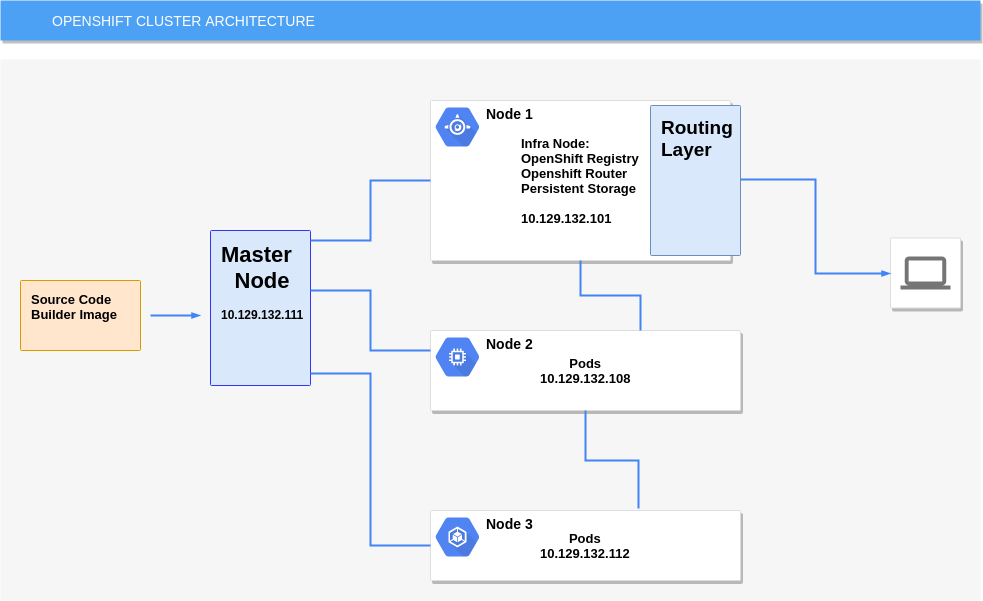
\includegraphics[scale = 0.5]{OpenShiftArchitecture}
    		\caption{Openshift cluster (Diagram Made using draw.io)}
    	  \end{center}
	  
	\end{figure}
	\pagebreak
	\section{Openshift Application Components}:
	\begin{itemize}
		\item 
		\textbf{Custom container images}:Each application deployment in OpenShift creates a custom container image to serve your application. This image is created using the application’s source code and a custom base image called a builder image.
		\ \\
		\ \\
		\textbf{Image streams}:Image streams are used to automate actions in Openshift. They consist of links to one or more container images. Using image streams, you can monitor applications and trigger new deployments when their components are updated.
		\ \\
		\textbf{Application pods}:OpenShift Online leverages the Kubernetes concept of a pod, which is one or more containers deployed together on one host, and the smallest compute unit that can be defined, deployed, and managed.
		\  \\
		\textbf{Build configs}:A build config contains all the information needed to build an application using its source code. This includes all the information required to build the application container image:
		\begin{itemize}
			\item  URL for the application source code
			\item Name of the builder image to use
			\item Name of the application container image that’s created
			\item Events that can trigger a new build to occur
		\end{itemize}
		\ \\
		\textbf{DeploymentConfigs}:If an application is never deployed, it can never do its job. The job of deploying and upgrading the application is handled by the deploymentconfigs component.
		\begin{itemize}
			\item  Currently deployed version of the application.
			\item Number of replicas to maintain for the application.
			\item Trigger events that can trigger a redeployment. By default, configuration.
			\item changes to the deployment or changes to the container image trigger an automatic application. redeployment
			\item Upgrade strategy. app-cli uses the default rolling-upgrade strategy.
		\end{itemize}
		\ \\
		\textbf{Deployments}:A deployment represents a unique version of an application. Each deployment references a version of the application image that was created, and creates the replication controller to create and maintain the pods to serve the application.\\
		\ \\
		\textbf{Services}:A service uses the labels applied to pods when they’re created to keep track of all pods associated with a given application.
	\end{itemize}
	\ \\
	\ \\
	\ \\
		\begin{figure}[h!]
    	\begin{center}
    	   	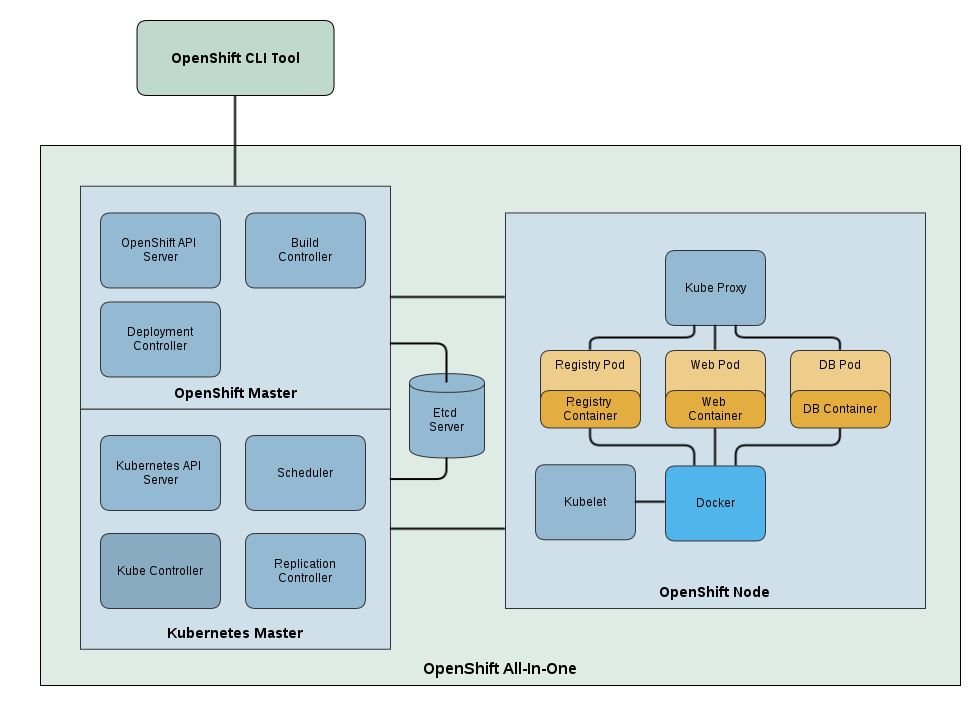
\includegraphics[scale=0.5]{openshiftallinone.png}
    		\caption{Openshift application components working together\cite{Appcomp}}
    	  \end{center}
	  
		\end{figure}
	\ \\
	\ \\
	
	\pagebreak
	\section{Openshift Installation}
	PreInstallation Step -
	4 systems are required out of which 1 is acting as master, 1 as infranode and other 2 as nodes.
	Configuration of these machines are:-
	\ \\
	\ \\
	\begin{table}[H]
		\begin{center}
		    \LARGE
			\begin{tabular}{|c|c|c|c|}
				\hline
				\textbf{Host Name} & \textbf{IP Address} & \textbf{CPUs} & \textbf{RAM} \\
				\hline
				master.cse.iitb.ac.in & 10.129.132.111 & 4 & 16GB  \\
				\hline
				node1.cse.iitb.ac.in & 10.129.132.101 & 4 & 8GB  \\
				\hline
				node2.cse.iitb.ac.in & 10.129.132.108 & 4 & 8GB  \\
				\hline
				node3.cse.iitb.ac.in & 10.129.132.112 & 4 & 2GB  \\
				\hline
				
			\end{tabular}
			\caption{Nodes}
		\end{center}
	\end{table}
	
	
	\textbf{Installation Steps}:
	\\
	\\
	Step 1: Set the hostname:
	
	hostnamectl set-hostname master.cse.iitb.ac.in ( For master node)
	\\
	\\
	Step 2: Configure /etc/hosts file for name resolution on all nodes
	\\
	\\
	Step 3: Update System on all node
	\\
	yum update -y
	\\
	\\
	Step 4: Install the following Packages on all nodes:  
	\\
	\\
	yum install -y wget git  nano net-tools docker-1.13.1 bind-utils iptables-services bridge-utils bash-completion kexec-tools sos psacct openssl-devel httpd-tools NetworkManager python-cryptography python-devel python-passlib java-1.8.0-openjdk-headless "@Development Tools"
	\\
	\\
	Step 5:Configure Ansible Repository on master Node only, in
	\\
	etc/yum.repos.d/ansible.repo
	\\
	\\
	Step 6:Start and Enable NetworkManager and Docker Services on all nodes
	\\
	\\
	Step 7:Install Ansible Package and Clone Openshift-Ansible Git Repo on Master Machine
	\\
	\\
	Step 8:Generate SSH Keys on Master Node and install it on all nodes
	\\
	\\
	Step 9:Now Create Your Own Inventory file for Ansible as following on master Node
	\\
	\\
	Step 10:Use the ansible playbook command to check the prerequisites to deply OpenShift Cluster on master Node
	\\
	\\
	Step 11:use the ansible playbook to Deploy OpenShift Cluster on master Node
	\\
	\\
	\textbf{ \href{https://docs.google.com/document/d/1-5IzdOLPmdm0L8KGBLJgSabSruhK_TCHPha0nX_jrXQ/edit?usp=sharing}{installation Document}}.
	\ \\
	\vspace{4cm}
	\ \\
	\textbf{Openshift web console}
	\ \\
	\ \\
	\begin{figure}[h!]
    	\begin{center}
    	   	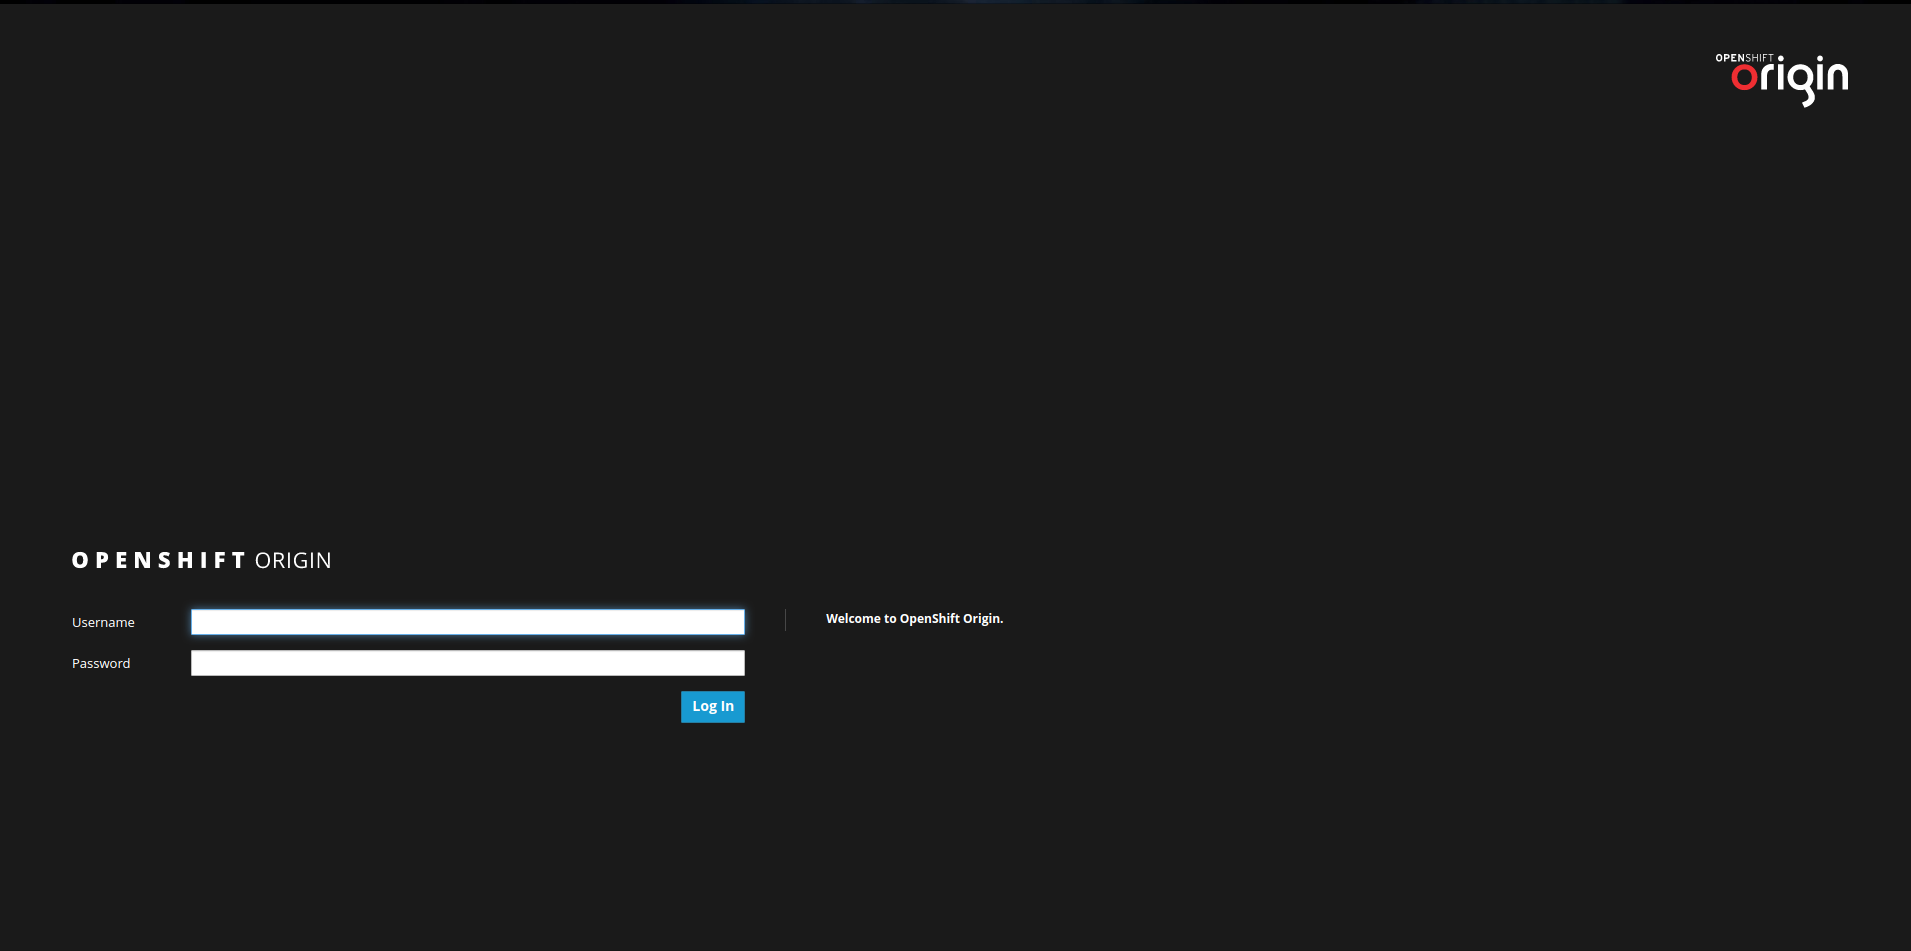
\includegraphics[width=18cm,height=16cm]{openshiftwebconsole.png}
    		\caption{Openshift web console}
    	  \end{center}
	  
	\end{figure}
	\ \\
	\pagebreak
	\ \\
	\begin{figure}[h!]
    	\begin{center}
    	   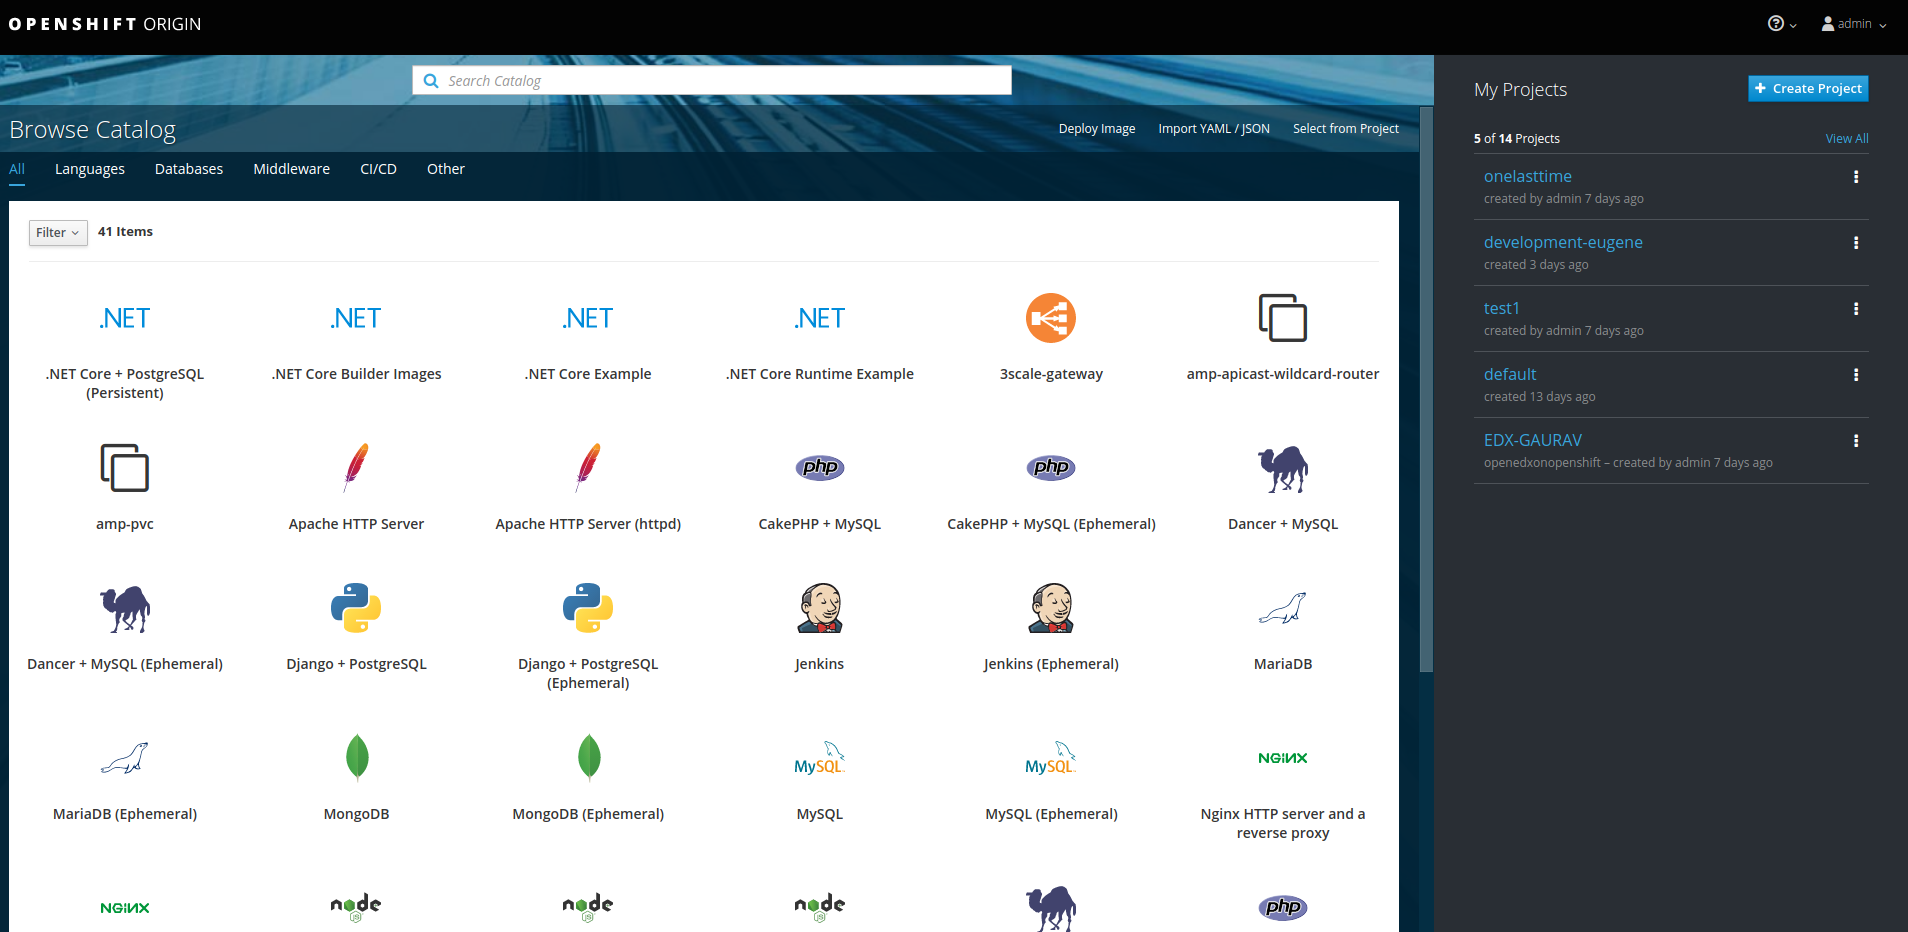
\includegraphics[width=18cm,height=18cm]{openshiftDashboard.png}
    		\caption{Openshift Dashboard}
    	  \end{center}
	  
	\end{figure}
	
	\chapter{Devstack Installation on Openshift}
	\section{Introduction}
	\large
	Devstack is the docker based installation of openedX.This chapter deals with the process of deployment of various services of openedX on openShift Cluster 
	
	\section{Setting up a persistent storage source}
	\begin{enumerate}
		\large
		\item \textbf{Installing the NFS server software}
		\begin{itemize}
			\item  yum -y install nfs-utils
		\end{itemize}
		\item \textbf{Configuring storage for NFS}
		\begin{itemize}
			\item  \textbf{To see all the block devices on master server}
			\ \\
			\# lsblk
			\item  \textbf{Creating a filesystem on your storage disk}
			\ \\
			\# mkfs.ext4 /dev/sda2
			
			
		\end{itemize}
		
		\item \textbf{Mounting your storage disk at startup}
		\begin{itemize}
			\item  \textbf{Creating a mountpoint directory}
			\ \\
			\# mkdir /var/nfs-data
			\item  \textbf{Getting your storage drive’s block ID}
			\ \\
			\# blkid
			\item  \textbf{Editing /etc/fstab to include your volume}
			\ \\
			\hfill
			
			
			
			
		\end{itemize}
			\begin{figure}[h!]
    	\begin{center}
    	   	
\includegraphics[scale = 0.34]{fstab.png}
    		\caption{/etc/fstab file}
    	  \end{center}
	  
	\end{figure}
		\begin{itemize}
			\item \textbf{Activating your new mount point}
			\ \\
			\# mount -a
			\ \\
			\# mount
		\end{itemize} 
		
		\item \textbf{Configuring NFS}
		\ \\
		\begin{itemize}
			\item \textbf{We'll need to export twenty five different NFS volumes.}
			\ \\
			\# mkdir -p /var/nfs-data/\{pv01,pv02,pv03,pv04,pv05..\}
			
			\item \textbf{Edit /etc/exports configration file to add all the volumes.}
			\ \\
			\ \\
	\begin{figure}[h!]
    	\begin{center}
    	   		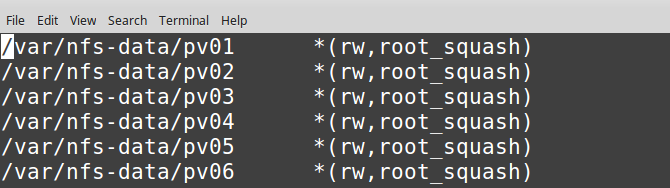
\includegraphics[scale=0.5]{pvolume.png}
    		\caption{/etc/exports}
    	  \end{center}
	  
	\end{figure}
			\ \\
			\ \\
			\item \textbf{Setting ownership of the mountpoint}
			\ \\
			\# chown -R nfsnobody.nfsnobody /var/nfs-data/
			\ \\
			\# chmod -R 0770 /var/nfs-data/
			\ \\
			\item \textbf{Setting firewall rules to allow NFS traffic}
			\ \\
			\# iptables -I INPUT -p tcp --dport 2049 -j ACCEPT
			\ \\
			\# service iptables save
			
		\end{itemize} 
		\ \\
		\item \textbf{Enabling and starting NFS}
		\begin{itemize}
			\item \textbf{Starting NFS services}
			\ \\
			for i in rpcbind nfs-server nfs-lock nfs-idmap;do systemctl restart \$i;done
			\ \\
			for i in rpcbind nfs-server nfs-lock nfs-idmap;do systemctl enable
			\item \textbf{Confirming that your NFS volume is exported and ready to use}
			\ \\
			\# exportfs
			
		\end{itemize} 
		
		
		\item \textbf{Creating a physical volume}
		\ \\
		To create a resource from a YAML template, use the oc create command along with
		the -f parameter, which specifies the template file you want to process.
		\ \\
		\textbf{
			\# oc --config /etc/origin/master/admin.kubeconfig create -f pv01.yaml
			\ \\
			persistentvolume "pv01" created}
		\ \\
		\ To\ get\ all\ active\ PVs\ on\ the\ server
		\# oc get pv
		\ \\
		\ \\
		\begin{figure}[h!]
    	\begin{center}
    	   			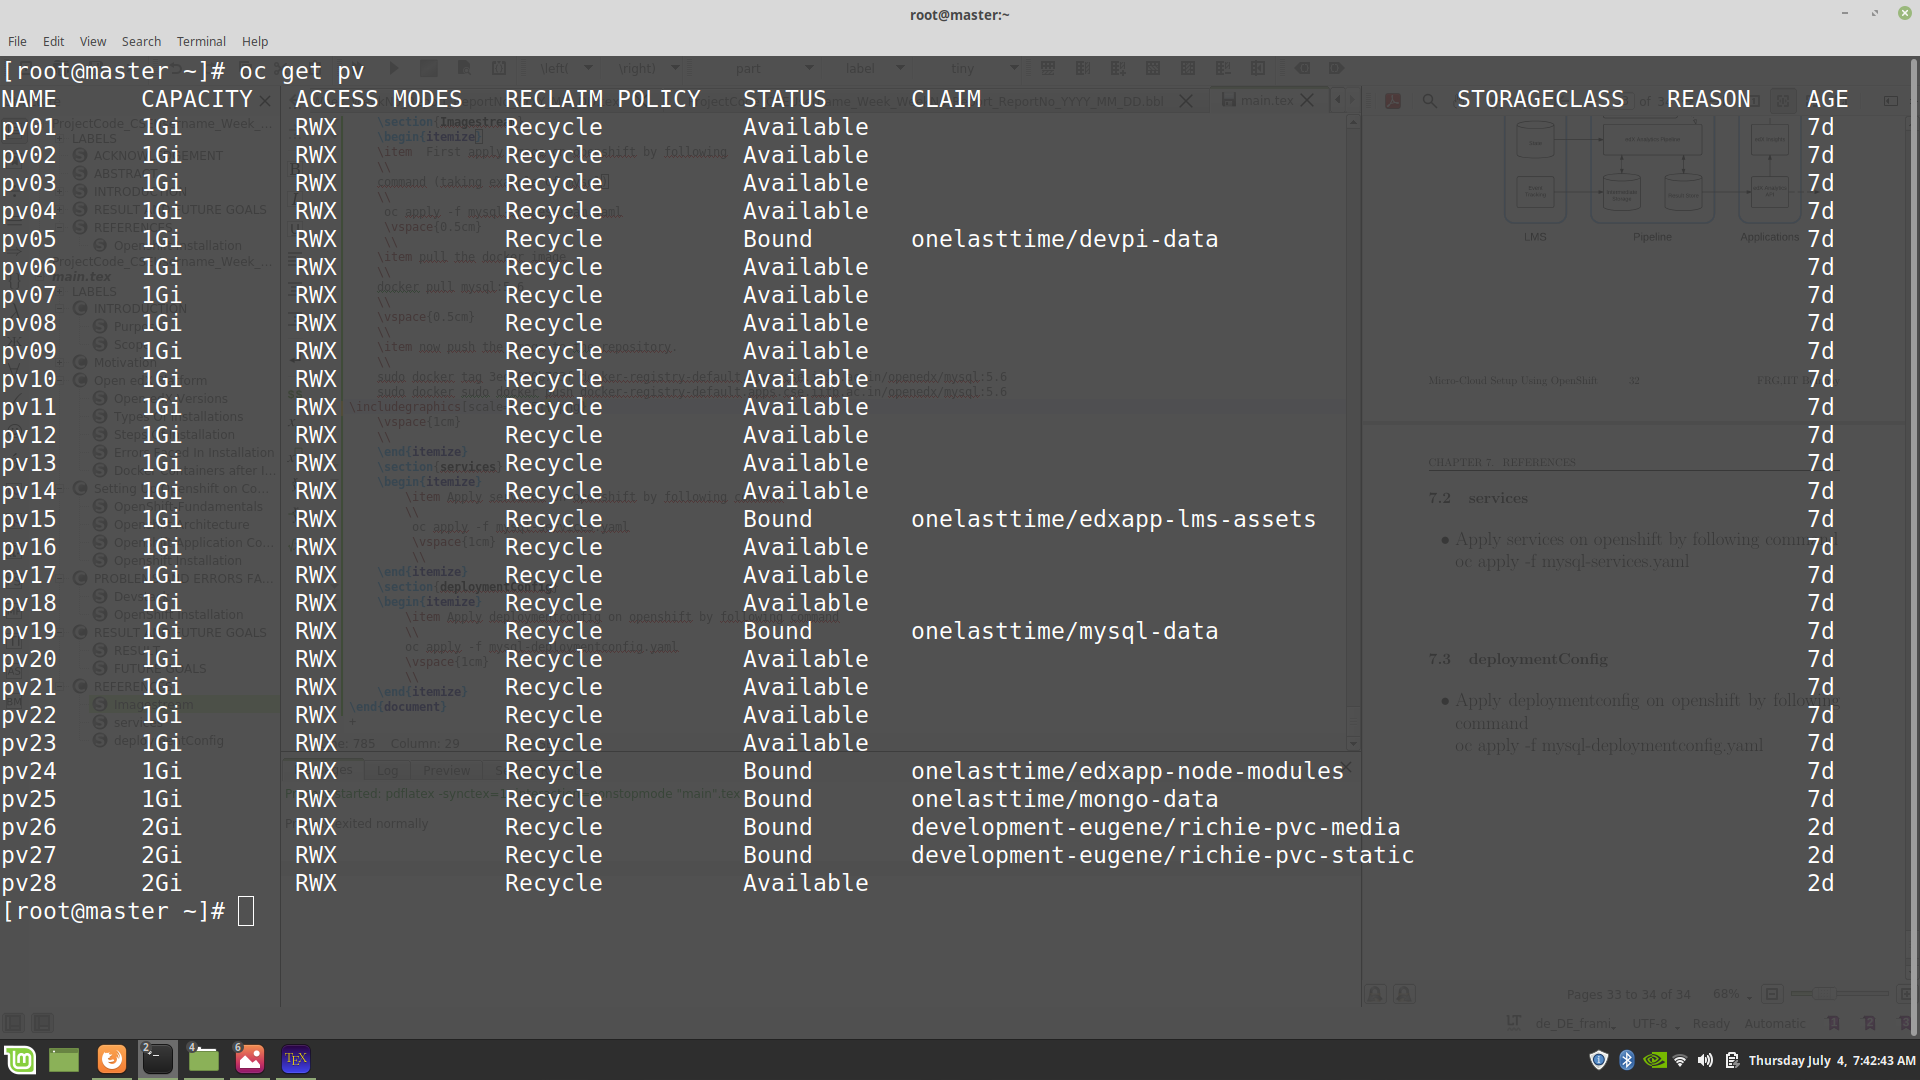
\includegraphics[width=16cm,height=16cm]{pv_image.png}
    		\caption{List of Persistent Volumes}
    	  \end{center}
	  
	\end{figure}
		
		
		
	\end{enumerate}
	
	\pagebreak
	\section{Storage binding to persistent volume}
	Persistent Volume Claims can be made after persistent volumes are created. \ \\
	The PVC can be created by using the yaml file. \ \\
	for example: \ \\
	oc apply -f devpi-data-persistentvolumeclaim.yaml \ \\
		\begin{figure}[h!]
    	\begin{center}
    	   		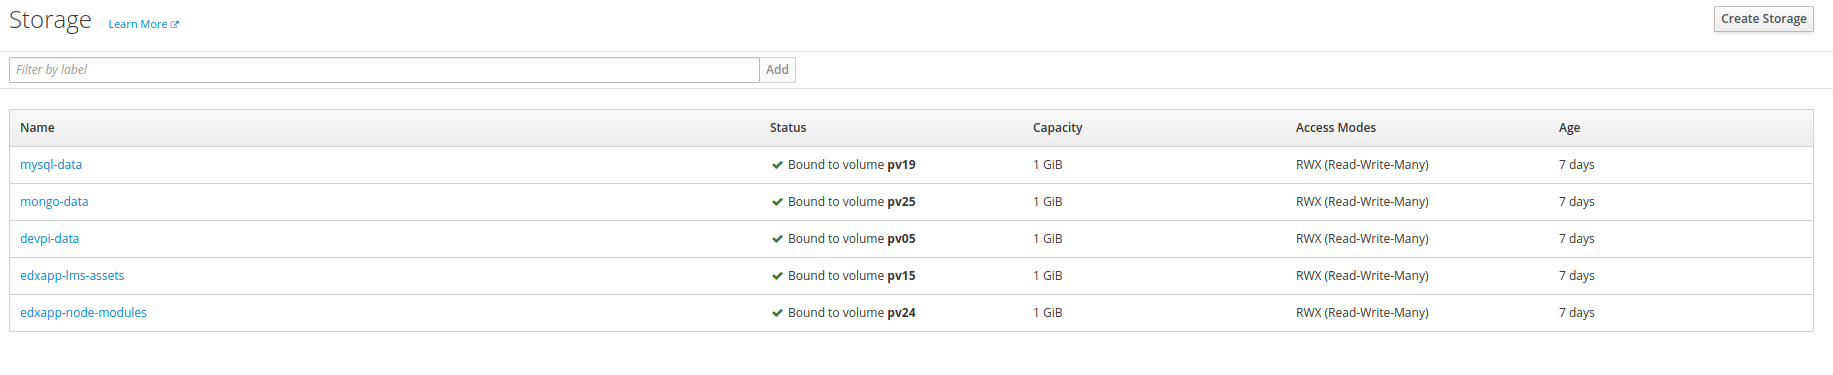
\includegraphics[scale=.55]{storagelist.png}
    		\caption{List Of PVC}
    	  \end{center}
	  
	\end{figure}
	\ \\
	\ \\
	\ \\
	\large
	\textbf{Storage Example}
	\ \\
	\ \\
		\begin{figure}[h!]
    	\begin{center}
    	   		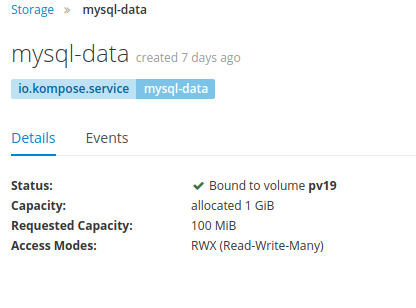
\includegraphics[scale=1]{storagexample.png}
    		\caption{mysql-data PVC}
    	  \end{center}
	  
	\end{figure}
	\pagebreak
	\large
	\section{Imagestream}
	Image streams are used to automate actions in Openshift. They consist of links to one or more container images. Using image streams, you can monitor applications and trigger new deployments when their components are updated.
	\begin{itemize}
		\item  First apply image on openshift by following 
		\\
		command (taking example of mysql)
		\\
		oc apply -f mysql-imagestream.yaml
		\vspace{0.5cm}
		\\
		\item pull the docker image
		\\
		docker pull mysql:5.6
		\\
		\vspace{0.5cm}
		\\
		\item now push the image to the repository.
		\\
		sudo docker tag 3ed1080b793f docker-registry-default.apps.cse.iitb.ac.in/openedx/mysql:5.6
		sudo docker sudo docker push docker-registry-default.apps.cse.iitb.ac.in/openedx/mysql:5.6
		\ \\
		\ \\
		\large
		\begin{figure}[h!]
    	\begin{center}
    	   		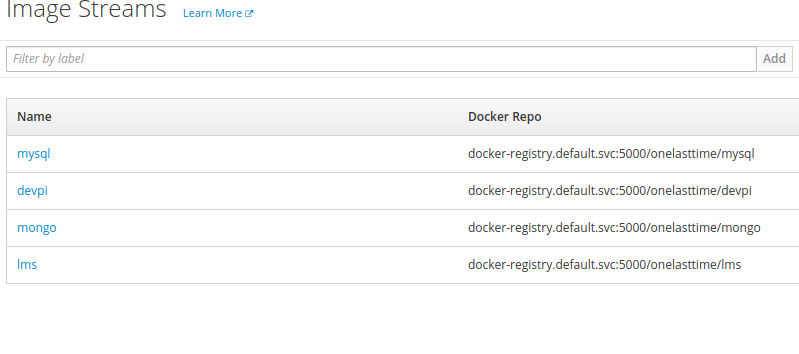
\includegraphics[scale=0.5]{imagelist.png}
    		\caption{Image Streams}
    	  \end{center}
	  
	\end{figure}
		\ \\
		\pagebreak
		\ \\
			\begin{figure}[h!]
    	\begin{center}
    	   			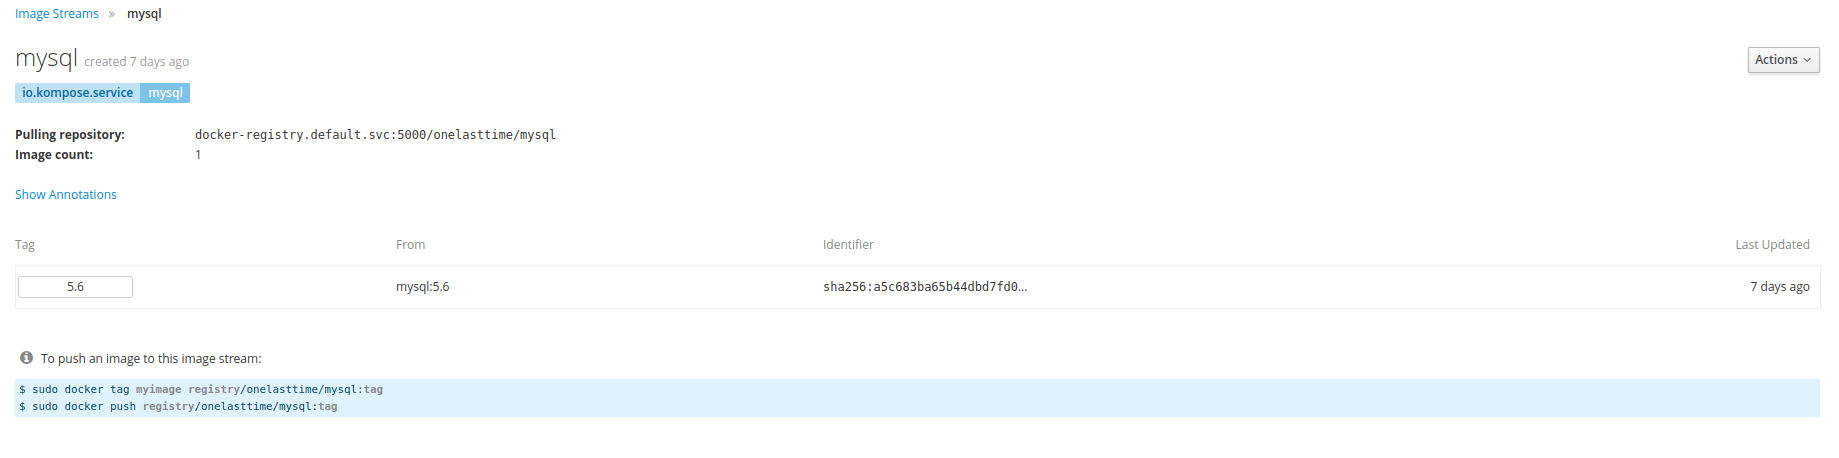
\includegraphics[width=16cm,height=8cm]{imagexample.png}
    		\caption{mysql Image Stream}
    	  \end{center}
	  
	\end{figure}
	
		
		\vspace{1cm}
		\ \\
	\end{itemize}
	\section{services}
	\begin{itemize}
		\item Apply services on openshift by following command
		\\
		oc apply -f mysql-services.yaml
		\ \\
		\ \\
		\begin{figure}[h!]
    	\begin{center}
    	   				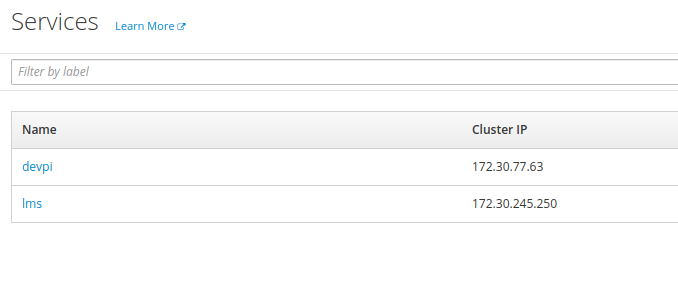
\includegraphics[scale=0.5]{servicelist.png}
    		\caption{Services}
    	  \end{center}
	  
	\end{figure}
		
		\ \\
		
			\begin{figure}[h!]
    	\begin{center}
    	   				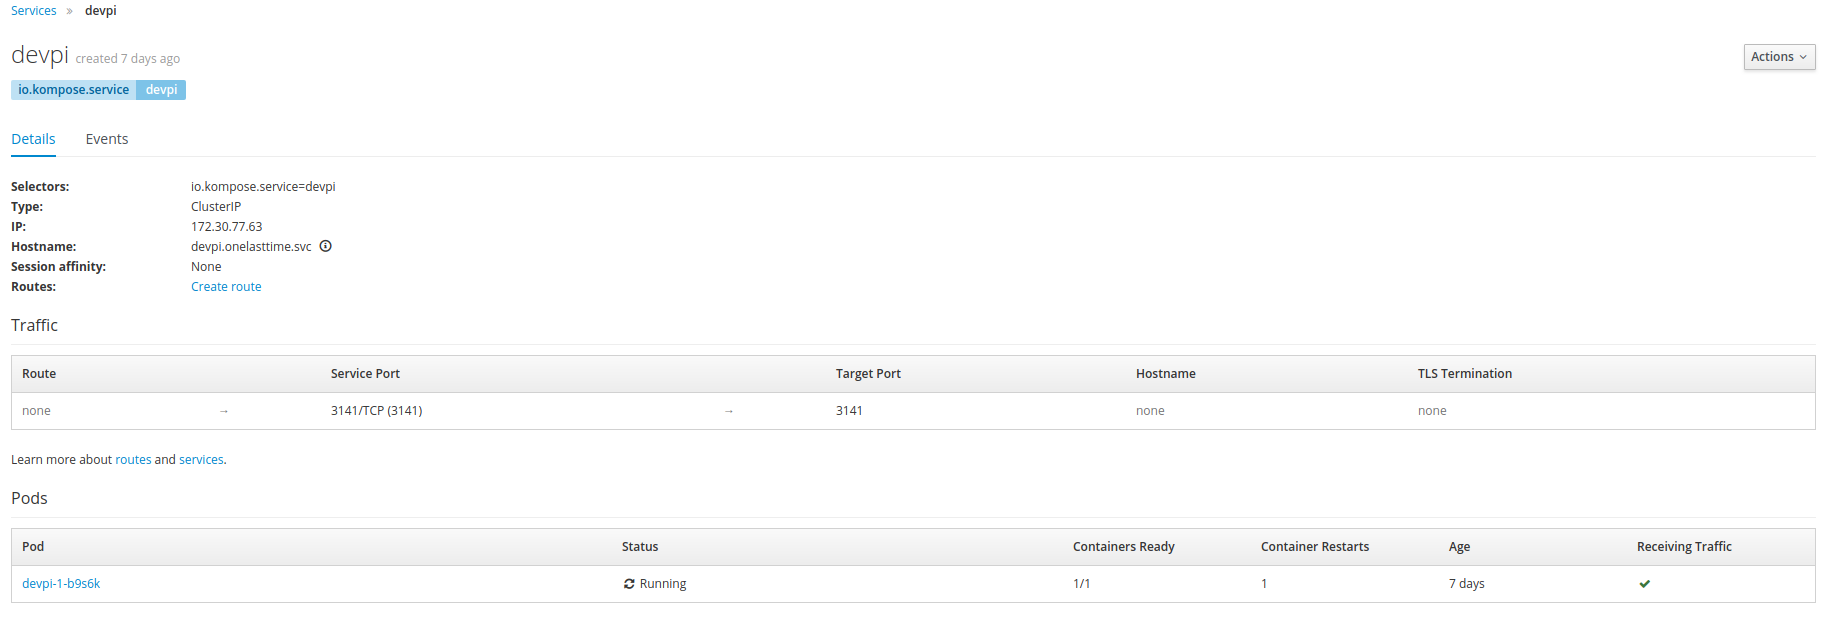
\includegraphics[width=16cm,height=10cm]{servicexample.png}
    		\caption{devpi service}
    	  \end{center}
	  
	\end{figure}
		\vspace{1cm}
	\	\\
	\end{itemize}
	\section{deploymentConfig}
	\begin{itemize}
		\item Apply deploymentconfig on openshift by following command
	\	\\
		oc apply -f mysql-deploymentconfig.yaml
		\ \\
		\begin{figure}[h!]
    	\begin{center}
    	   				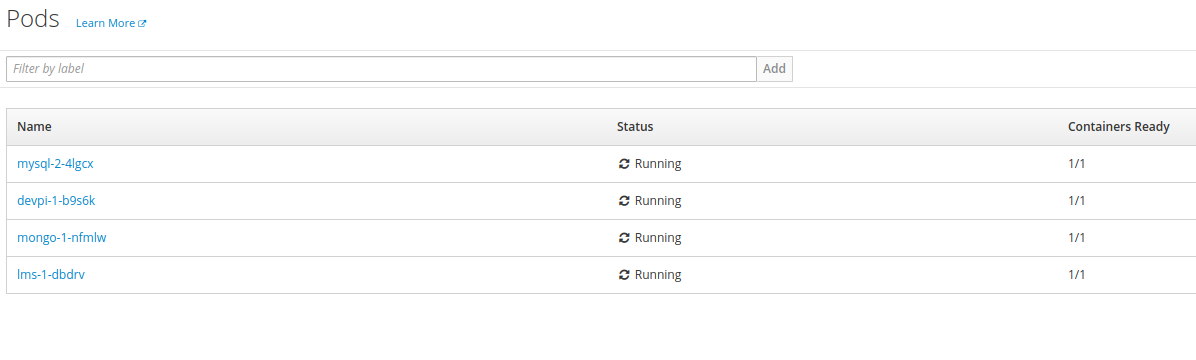
\includegraphics[width=16cm,height=6cm]{pod.png}
    		\caption{List of deployment}
    	  \end{center}
	  
	\end{figure}
				
		\ \\
			\begin{figure}[h!]
    	\begin{center}
    	   				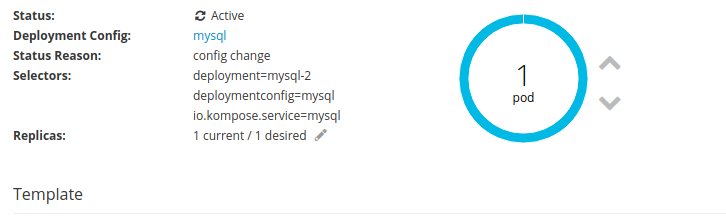
\includegraphics[scale=0.5]{podxample}
    		\caption{mysql deployment}
    	  \end{center}
	  
	\end{figure}
	
		
		\ \\
	\end{itemize}
	\chapter{PROBLEMS AND ERRORS FACED}
	\section{Devstack}
	\large
	\begin{itemize}
		\item \textbf{./provision.sh: line 21: /usr/local/bin/docker-compose: Permission denied} \ \\
		Makefile:59: recipe for target 'dev.provision.run' failed \ \\
		make: *** [dev.provision.run] Error 126 \ \\
		Solution : \ \\
		$ sudo -i  \ \\
		$ curl -L \ \\ https://github.com/docker/compose/releases/download/1.18.0/docker-compose-`uname -s`-`uname -m` -o /usr/local/bin/docker-compose \ \\
		$ chmod 755 /usr/local/bin/docker-compose \ \\
		$ exit \ \\
		
		\item \textbf{TASK [common : Update expired apt keys] **************} \ \\
		This error occurs due to the fetching to apt-keys from an expired link. \ \\
		Solution : \ \\
		1.sudo exec -it edx.devstack.lms bash \ \\
		2.cd app/edx\_ansible/edx\_ansible/playbooks/roles/common\_vars/defaults/ \ \\
		3.vi main.yml \ \\
		4.On entering the main.yml file in vim editor change the link for the keyword
		COMMON\_EDX\_PPA\_KEY from keyserver.ubuntu.com to  hkp://keyserver.ubuntu.com:80 \ \\
	\end{itemize}
	
	\section{OpenShift Installation}
	\begin{itemize}
		\item \textbf{wget-1.14-18.el7\_6.1.x86\_64:No more mirrors to try.} \ \\
		Fix: sudo yum install wget \ \\
		\item \textbf{TLS Handshake Error/Connection Timed out} \ \\
		Fix: Run the command again. \ \\
		\ \\
		\item  \textbf{API Server Error:Get https://127.0.0.1:8443/healthz?timeout=32s:} \ \\
		Connect : connection refused ()
		Probable Reason:
		Lower Resources on PC (Weak VM): \ \\
		(Encountered This Error when installation was done on Single Machine Using VMs)
		\ \\
		Fix: used 4 dedicated machines for multi-node installation.
		\item \textbf{Error :- Starting openshift.io/sdn \ \\
			IP: 10.128.0.0 conflicts with host network : 10.129.132.0/24
		}
		\ \\
		While Running deploy\_cluster.yml \ \\
		In the task Running Handler [openshift\_master:restart master-controllers] \ \\
		Resolution \ \\  vi /etc/origin/master/master-config.yaml \ \\ 
		under networkconfig- \ \\
		change clusternetwork CIDR from 14 to 16. \ \\ 
		
		
	\end{itemize}
	
	\chapter{RESULT AND FUTURE GOALS}
	\section{RESULT}
	\large
	In the project Micro-Cloud setup using Openshift, we have
	\begin{itemize}
		\vspace{0.3cm}    
		\item Configured system hardware according to the Openshift requirement of setup involving one master and 3 nodes.
		\vspace{0.3cm}    
		\item Successfully setup a system consisting of 4 machines, one serving as master and other 3 as nodes.
		\vspace{0.3cm}
		\item Installed Openshift on local server with 1 master, 1 infra node and 2 nodes.
		\vspace{0.3cm}
		\item Accessed openshift through terminal as well as openshift console i.e.
		\textbf{ \href{https://master.cse.iitb.ac.in:8443}{master-console}}.
		\vspace{0.3cm}
		\item Successfully build and deployed various applications based on Ruby,PHP, NodeJs etc.
		\vspace{0.3cm}
		\item Did Successful Scaling and Descaling of pods.
		\vspace{0.3cm}
		\item Tried Installation of OpenEdx platform on openshift cluster.
		\vspace{0.3cm}
		\item Deployed various services of open-edx like mysql,mongodb,
		chrome,lms,cms etc on openshift.
		\large
	\end{itemize}
	\vspace{0.6cm}
	\pagebreak
	\Large
	\section{FUTURE GOALS}
	\Large
	\begin{itemize}
		\item Complete deployment of open-edx on openshift by resolving conflicts, being faced in provisioning.
		\vspace{0.3cm}
		\item  Installation of open-edx on openshift, using Arnonld tool.
		\\
		here is github repository for Arnold
		\textbf{ \href{https://github.com/openfun/arnold}{Arnold-openshift}}.
		\vspace{0.3cm}
		\item Openshift installation on multiple machines.
	\end{itemize}
	\pagebreak
	\textbf{REFERENCES}
	\large
	\begin{itemize}
		\item The github link for all documentations related to project is
		\\
		\textbf{\href{https://github.com/fresearchgroup/Micro-Cloud-setup-using-Openshift-on-commodity-servers}{	https://github.com/fresearchgroup/Micro-Cloud-setup-using-Openshift-on-commodity-servers}}.
		\ \\
		
		\vspace{0.5cm}
		
		\item The Origin Community Distribution of Kubernetes that powers Red Hat Openshift.
		\\
		\textbf{ \href{https://www.okd.io/}{https://www.okd.io/}}.
		\vspace{0.5cm}
		\item Setting up of openshift in multinodes.
		\\
		\textbf{ \href{https://youtu.be/JhlzSoayksY}{https://youtu.be/JhlzSoayksY}}.
		\vspace{0.5cm}
		\item Complete steps to install openshift
		\\
		\textbf{\href{https://github.com/fresearchgroup/Micro-Cloud-setup-using-Openshift-on-commodity-servers}{https://github.com/fresearchgroup/Micro-Cloud-setup-using-Openshift-on-commodity-servers}}
		\vspace{0.5cm}
		\item Deploying open-edx using Arnold
		\\
		\textbf{ \href{https://github.com/openfun/arnold}{https://github.com/openfun/arnold}}.
		\vspace{0.5cm}
		\item Openshift in Action by Jamie Duncan, John Osborne.
		\item Image Sources \ \\
		Fig. 1:http://http://protoinformatico.com/"Accessed on July 4 2019"
		\ \\
		Fig. 2:https://en.wikipedia.org/wiki/Docker\_(software)"Accessed on July 4 2019"
		\ \\
		Fig. 3:https://www.mindfireit.com/cyber-security/introduction-to-container-services/attachment/introduction-to-container-services-docker-kubernetes-openshift-configuration-code-runtime-engine/"Accessed on July 4 2019"
		\ \\
		Fig. 4:https://blog.docker.com/2018/09/join-the-beta-for-docker-engine-18-09/docker-website-2018-diagrams-071918-v5\_a-docker-engine-page-first-panel-2/"Accessed on July 4 2019"
		\ \\
		Fig. 5:https://cdn-images-1.medium.com "Accessed on July 4 2019"
		\ \\
		Fig. 6:https://techbeacon.com "Accessed on July 4 2019"
		\ \\
		Fig. 7:https://www.networkslayer.com/ingress/ "Accessed on July 4 2019"
		\ \\
		Fig. 8:https://image.slidesharecdn.com "Accessed on July 4 2019"
		\ \\
		Fig. 10:https://blog.openshift.com/openshift-v3-deep-dive-docker-kubernetes/ "Accessed on July 4 2019"
		
		
		
		\bibliographystyle{ieeetr}
        \bibliography{biblio}
		
	\end{itemize}
	
	\begin{center}
		
	\end{center}
	\pagebreak
\end{document}
+